\documentclass{article}

\usepackage{cite}

\usepackage[preprint]{neurips_2020}
\usepackage[utf8]{inputenc} % allow utf-8 input
\usepackage[T1]{fontenc}    % use 8-bit T1 fonts
\usepackage{hyperref}       % hyperlinks
\usepackage{url}            % simple URL typesetting
\usepackage{booktabs}       % professional-quality tables
\usepackage{amsfonts}       % blackboard math symbols
\usepackage{nicefrac}       % compact symbols for 1/2, etc.
\usepackage{microtype}      % microtypography
\usepackage{graphicx}
\usepackage{float}

\title{Machine Learning Project Interim Report: Mechanisms of Action (MoA) Prediction}

\author{
    Malte Meng, 2020280441 (Leader) \\
    \AND 
    Khang Hui Chua, 2020280442 \\
    \AND
    Kai Wen Yoke, 2020280598
}


\begin{document}
\maketitle
\begin{abstract}
This interim report documents the methods we have tried so far for the MoA Kaggle competition (\url{https://www.kaggle.com/c/lish-moa/}). This is a multi-label classification task, where we are to predict the probabilities of each of 206 mechanisms of action (MoAs) of a drug sample, given tabular data on gene expression and cell viability levels of cell samples treated with that drug sample. We tried various feature engineering methods, model architectures, training strategies and evaluation methods, and have currently achieved 109th position out of 4081 teams. This was achieved by blending three different models together, with the best individual model achieving 500th position. With ten days left for the competition (ending 30 Nov), there are still several architectures we would like to try, and if they perform well individually they will be added into our model blend. 
\end{abstract}

\newpage
\tableofcontents
\newpage

\section{Overview of the Kaggle competition: MoA Prediction }
For our Machine Learning project, we chose a currently active Kaggle competition "Mechanisms of Action (MoA) Prediction" that ends on 30th November: \url{https://www.kaggle.com/c/lish-moa/}. 

\subsection{Problem Statement}
Given data on gene expression and cell viability levels of cell samples in response to being treated by a drug sample at a particular dosage and for a particular time duration, the task is to predict the MoA of the drug. This is a multi-label classification task, as each drug sample can be associated with more than one MoA. The accuracy of solutions will be evaluated on the average value of the logarithmic loss function applied to each drug-MoA pair.

\subsection{Dataset overview}
We have 23814 data samples in the training set. The entire dataset includes roughly 5000 unique drugs, with each drug profiled multiple times at different dosages and treatment times. 

\subsubsection{Raw features}
The raw data features are shown in Figure \ref{fig:raw_data}. 

\begin{figure}[H]
\begin{center}
	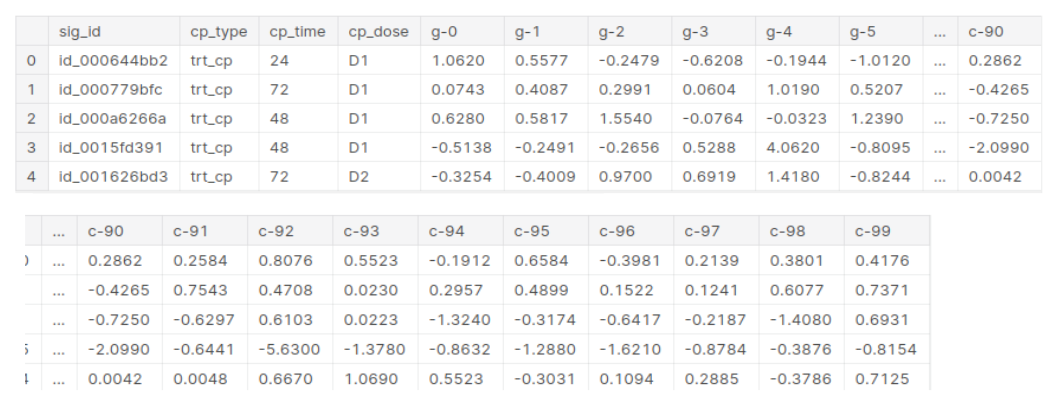
\includegraphics[width=1\textwidth]{pics/raw_data.png}
    \caption{Raw data features}
\label{fig:raw_data}
\end{center}
\end{figure}

There are 772 \textbf{gene expression features}, with each gene feature representing the expression level of a particular gene, and 100 \textbf{cell viability features}, with each cell viability feature representing the viability of one cell line, meaning that there are 100 cell lines in this dataset. The actual names of the gene features and cell types are hidden, so a hand-crafted approach would not be possible. The \textbf{cp\_type} attribute indicates whether a data sample is treated with a drug (\texttt{trt\_cp}) or a control (\texttt{ctl\_vehicle}), and a control sample would have no associated MoAs, but note that there are data samples which are not controls and also do not belong to any of the 206 MoAs that are our target labels tested during scoring. The \textbf{cp\_dose} is a binary feature and comprises two levels of dosage D1 or D2, and \textbf{cp\_time} is a categorical feature comprising three treatment durations (24, 48 or 72 hours). 

\subsubsection{Target labels}
The frequency of each of the 206 MoA target labels across the train dataset are shown in Figure \ref{fig:scored_labels}. 

\begin{figure}[H]
\begin{center}
	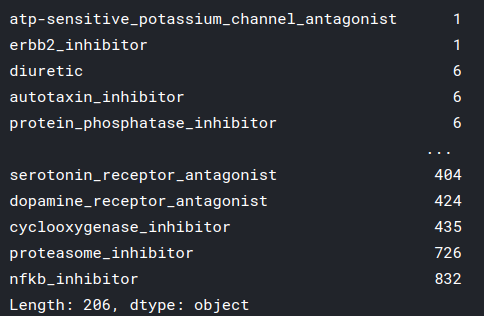
\includegraphics[width=0.7\textwidth]{pics/scored_labels.png}
    \caption{Frequency of each of the 206 MoA target labels in training data}
\label{fig:scored_labels}
\end{center}
\end{figure}

The classes in the dataset are highly imbalanced as many of the target MoAs have only one entry each while some have hundreds. The train dataset also contains an additional non-scored 402 target MoAs for each data sample, meaning that we do not have to predict these auxiliary MoAs for the test dataset.


\section{Methods and experimentation}
Much useful information has been discussed on the Kaggle competition discussion boards. Many public notebooks have also been shared. We leverage on these resources for our experimentation process. We found feature engineering, model architectures, training strategies, evaluation methods and model blending having the greatest influence over our performance on the leaderboard, and below we will discuss further the different methods we tried.

\subsection{Feature Engineering}
Preprocessing and feature engineering is essential in this competition where tabular data is involved, unlike unstructured data such as images, audio and text, where deep learning can directly be applied to automatically extract features. This is because the given tabular data has heterogeneous features, some categorical, some numerical and also with different units and scaling. Furthermore, the features are also sparse with sometimes little variation in a column of the table. These lead to features in a high-dimensional space that is not dense and continuous, which makes it difficult for us to exploit NNs which have proven to be one of the most successful ML models. Below, we discuss feature preprocessing methods to make the data more amenable to NNs.

\subsubsection{Raw features}
The raw features of the dataset include categorical and numerical ones. Categorical features are \textbf{cp\_type} (drug or control sample), \textbf{cp\_dose} (low or high dosage) and \textbf{cp\_time} (24, 48 or 72 hours). Numerical ones are the 772 \textbf{gene expression features} and the 1000 \textbf{cell viability features}. 

\subsubsection{One hot encoding of categorical features}
The categorical features \textbf{cp\_dose} and \textbf{cp\_time} are one-hot encoded, while only data samples with \textbf{cp\_dose} == \texttt{trt\_cp} are retained. The control group is removed because when \textbf{cp\_dose} == \texttt{ctl\_vehicle}, the cell samples are not treated with any drugs so there are no associated MoA target labels.

\subsubsection{Standardisation of numerical features}
The raw gene expression and cell viability data given by the organisers already went through quantile normalisation to standardize the shape of the distributions on each plate. However, the data is also clipped at -10 and 10, resulting in spikes at these two points (see Figure \ref{fig:raw_distrib}). There are also outliers that occur far from the mean of the normal distributions. Therefore, we still apply \texttt{QuantileTransformer} from \texttt{scikit-learn} with 100 quantiles to transform the given raw data into normal distributions with range from -1 to 1. Furthermore, it has been empirically shown that machine learning models work better with standardized normally distributed data.

\begin{figure}[H]
\begin{center}
	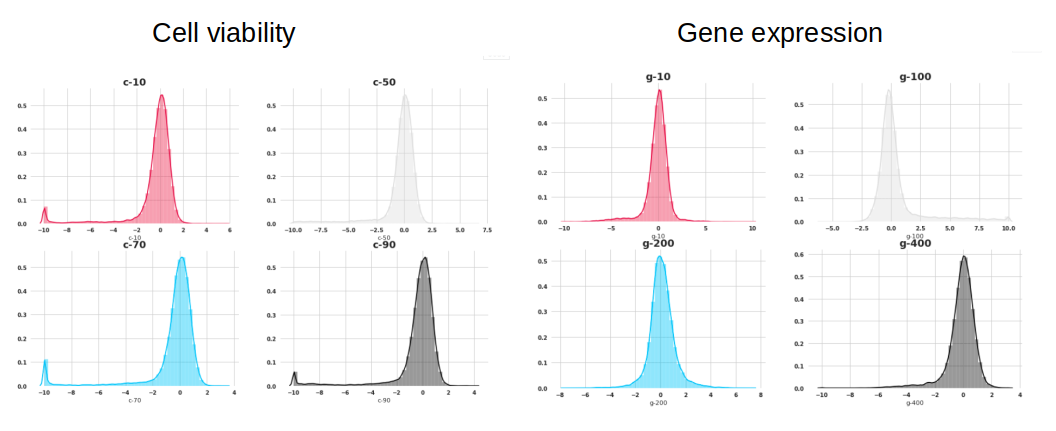
\includegraphics[width=1\textwidth]{pics/raw_distrib.png}
    \caption{Distribution of a few cell viability and gene expression data features clipped at -10 to 10}
\label{fig:raw_distrib}
\end{center}
\end{figure}

\subsubsection{Dimensionality reduction of numerical features}
Data exploration reveals many correlations between different gene expression features and cell viability features (see Figure \ref{fig:correlation_num}). 

\begin{figure}[H]
\begin{center}
	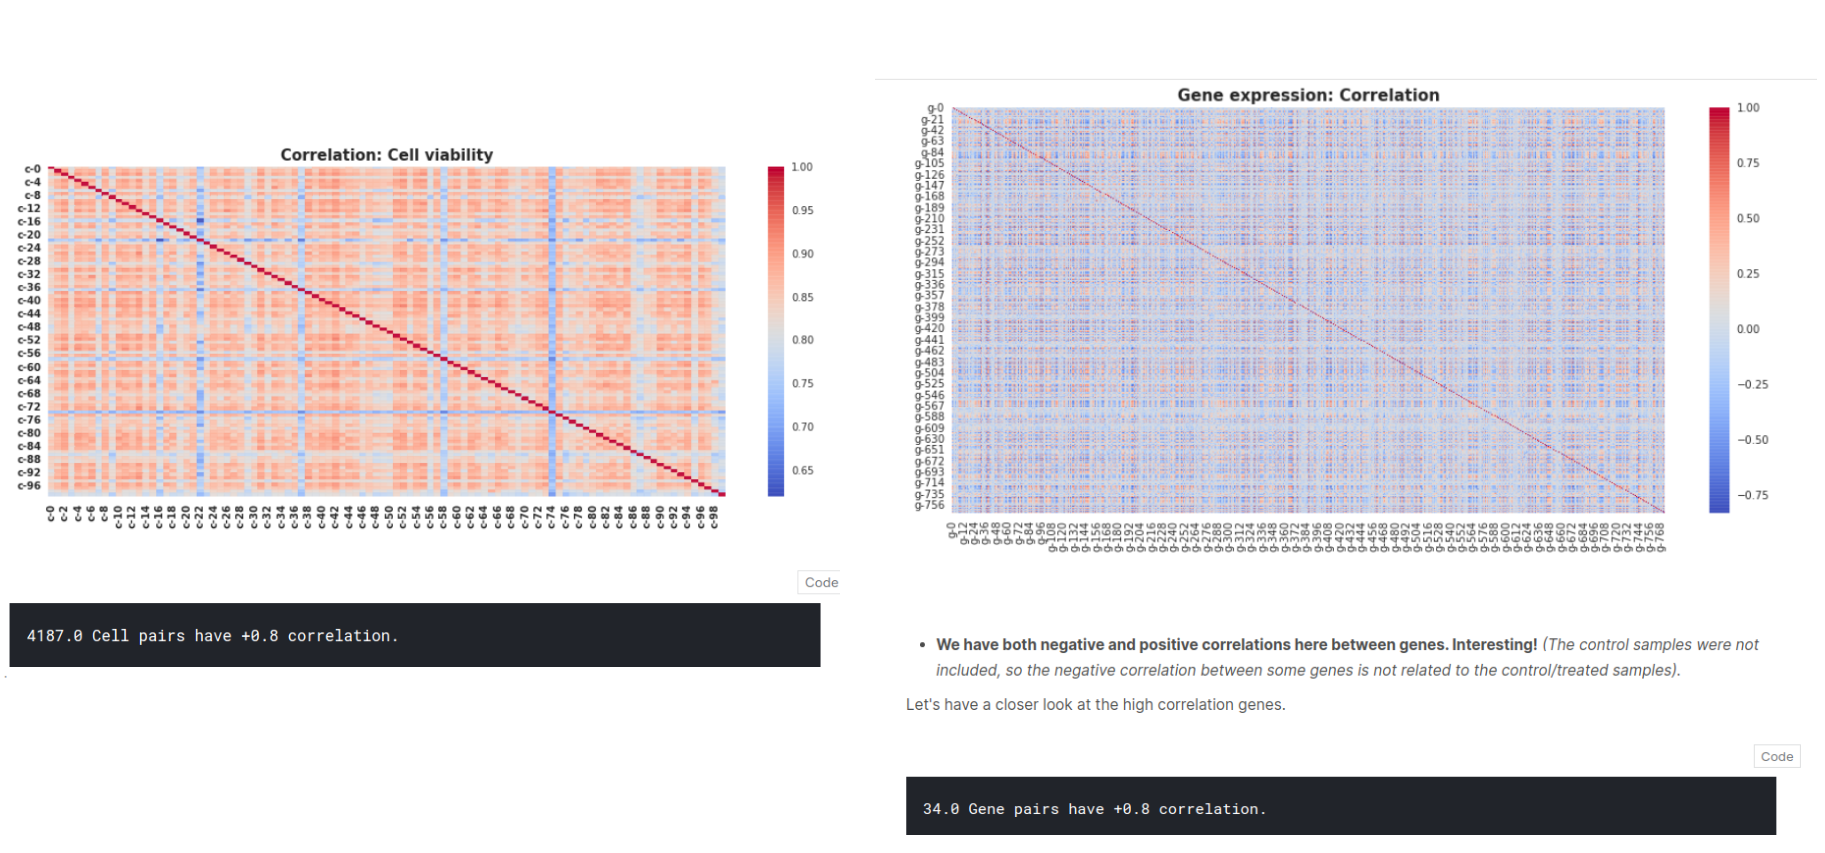
\includegraphics[width=1\textwidth]{pics/correlation_num.png}
    \caption{Correlations among cell viability and gene expression features}
\label{fig:correlation_num}
\end{center}
\end{figure}

This suggests that many features are redundant and thus the dimensionality of features can be reduced. We achieve this by using PCA, variance thresholding, Kmeans clustering, and statistics-based aggregation. 

\begin{enumerate}
    \item \textbf{PCA}: We applied \texttt{PCA} from \texttt{scikit-learn} with 600 components for gene expression features and 50 components for cell viability features. These are the number of components required to explain 95\% of the cumulative variance of the gene expression and cell viability features respectively. PCA works by summarising the correlations between different features into fewer principal components.
    
    \item \textbf{Variance thresholding}: We remove numerical features that have variance less than 0.87 (arbitrary) before applying Kmeans clustering and statistics-based aggregation. The rationale is that if many data samples share similar values for a certain feature, then the feature is not going to be very good at distinguishing between the different data samples.
    
    \item \textbf{Kmeans clustering}: We applied \texttt{KMeans} from \texttt{scikit-learn} to cluster the data samples into 22 clusters based on their gene expression features, and 5 clusters based on their cell viability features. The gene and cell cluster IDs of each data sample is then one-hot encoded. The number of clusters were arbitrarily chosen by visualising the clusters using \texttt{TSNE} (t-distributed Stochastic Neighbor Embedding) from \texttt{scikit-learn} as seen in Figure \ref{fig:tsne9}.

\begin{figure}[H]
\begin{center}
	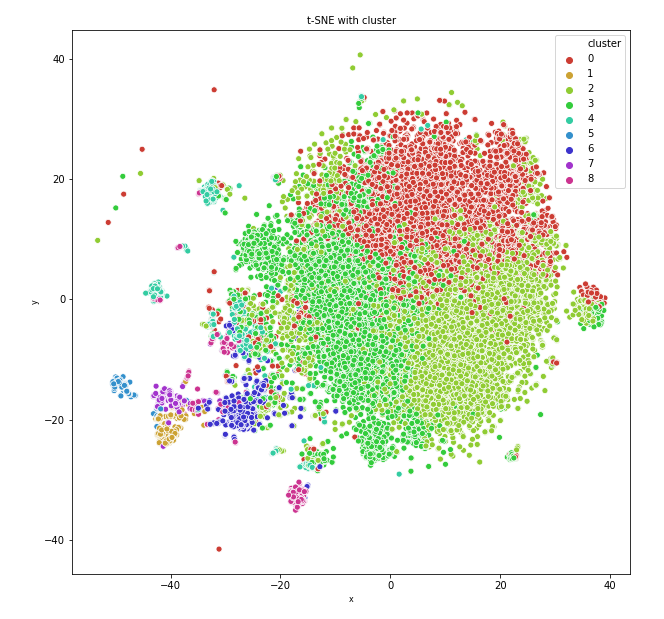
\includegraphics[width=0.6\textwidth]{pics/tsne9.png}
    \caption{t-SNE visualisation plot of gene expression features with 9 clusters}
\label{fig:tsne9}
\end{center}
\end{figure}

    \item \textbf{Statistics-based aggregation}: We also created more features from the raw gene and cell features based on statistics, such as sum, mean, standard deviation, kurtosis, skew and square across all gene features and across all cell features respectively, as a way of combining all gene features into a few representative statistics and all cell features into a few representative statistics.
\end{enumerate}

\subsection{Model experimentation}
Most of the more successful models use neural architectures. Nevertheless, the idea is to get as diverse models as possible to boost our final ensemble.

\subsubsection{Fully connected networks}
We tried implemnting simple fully connected networks with \texttt{pytorch} experimenting with various number of hidden layers, number of neurons, batch normalisation, dropout rates, weight and bias initialisations, activation functions (\texttt{ReLU, LeakyReLU, Swish}) and loss functions. 

\subsubsection{TabNet}
Other than vanilla fully connected networks, we also tried more novel architectures such as TabNet \cite{tabnet} using the \texttt{pytorch\_tabnet} library which is designed specifically for tabular data with an attention mechanism that learns a sparse mask over input features. 

\subsubsection{Other model architectures}
We are also planning to try CNN architectures and also other non-NN architectures such as K-NN.  Nevertheless, so far the best performing single model is the simple fully connected network with architecture shown in Figure \ref{fig:fcn}, with batch normalisation, dropout, \texttt{kaiming\_normal} weight initialisation, bias initialisation for the final layer corresponding to the frequency of each target label in the training set, \texttt{ReLU} activation and \texttt{BCEWithLogitsLoss} with label smoothing. This combination of parameters helps to speed up convergence and regularise the training process, especially when considering the label imabalance for the training set.

\begin{figure}[H]
\begin{center}
	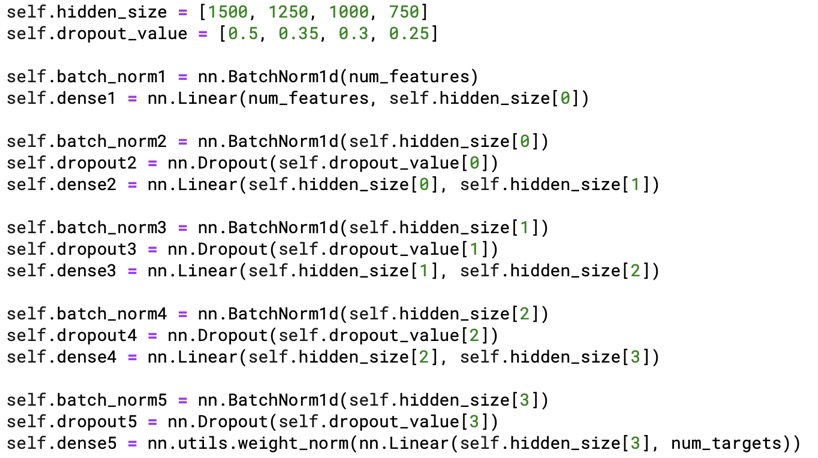
\includegraphics[width=1\textwidth]{pics/fcn.JPG}
    \caption{Best fully connected network architecture currently}
\label{fig:fcn}
\end{center}
\end{figure}


\subsection{Training strategies involving unscored target labels}
Other than the conventional way of training the models on the training data and using the trained model to predict the labels of the test data, we also tried other training strategies involving the use of the 402 unscored target labels. This includes using the unscored target labels as meta-features and for transfer learning. Unscored target labels are useful because they share significant correlation with scored target labels, as seen in Figure \ref{fig:scored_unscored_corr}, therefore having information about the unscored target labels could help us predict the scored labels of the test data samples.

\begin{figure}[H]
\begin{center}
	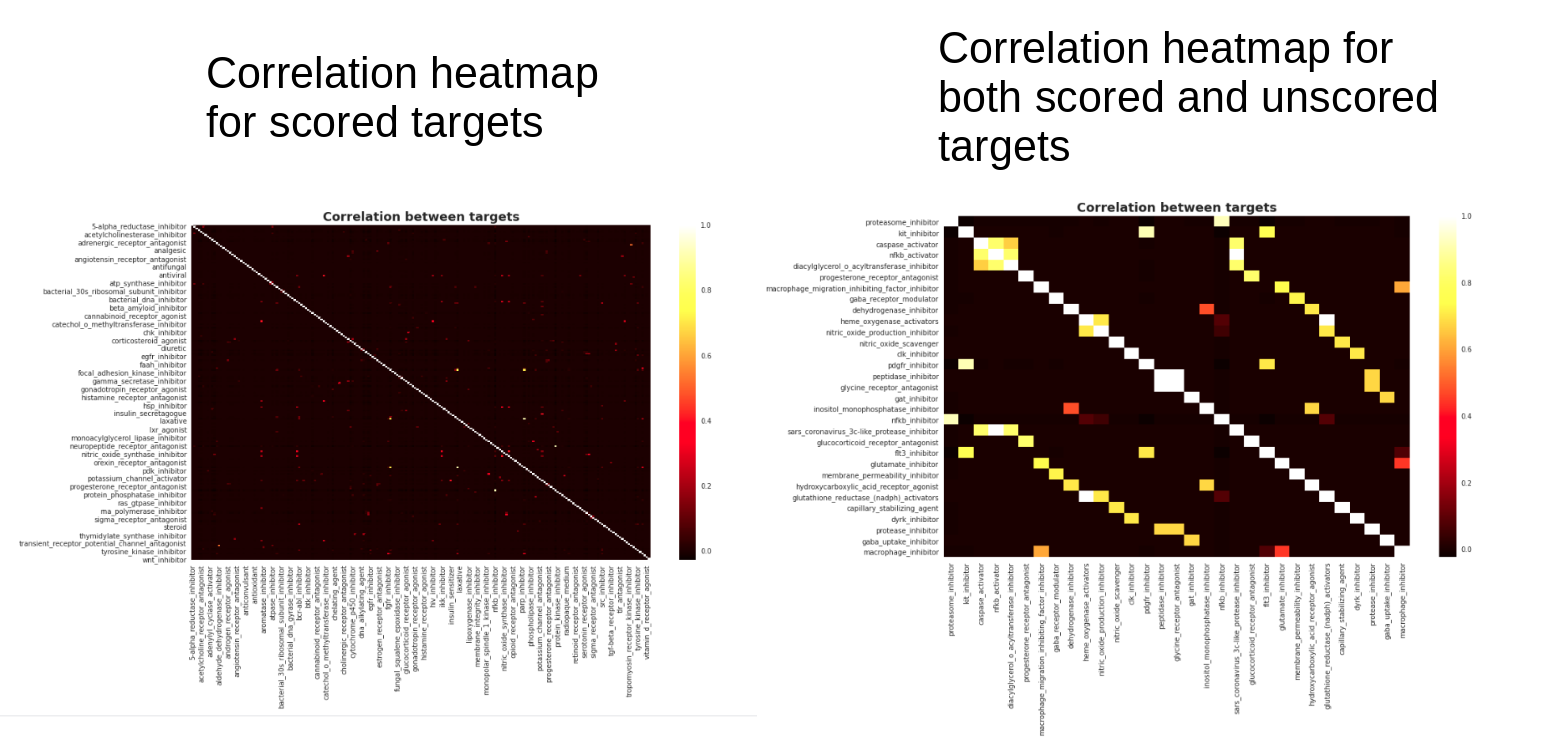
\includegraphics[width=1\textwidth]{pics/scored_unscored_corr.png}
    \caption{Correlation heatmap of scored target labels only VS correlation heatmap of both scored and unscored target labels combined}
\label{fig:scored_unscored_corr}
\end{center}
\end{figure}

\subsubsection{Unscored target labels as meta-features}
The idea is to first train a fully connected network to predict the 402 unscored target labels of the training dataset, then use the trained network (say \texttt{model\_1}) to predict the unscored target labels of the test dataset. Note that \texttt{model\_1} has 402 neurons in the last layer corresponding to the unscored target labels. Then, we train a second model \texttt{model\_2}, which has 206 neurons in the last layer corresponding to the scored target labels. In addition, \texttt{model\_2} also has the unscored target labels predicted by \texttt{model\_1} as input. We call these predicted unscored target labels 'meta-features' that help improve model performance. 

\subsubsection{Transfer learning: Unscored target labels for pretraining}
The idea is we first pretrain a fully connected network with 206+402=608 neurons in the last layer by utilising both the scored and unscored target labels. Then, we freeze the weights in the top layers, replace the last layer with a layer of only 206 neurons, and train the same model again with only the weights in the last layer being tuned, and only the 206 scored target labels involved. This method has also been quite successful.

\subsection{CV Evaluation}
In the competition, submissions are scored by the log loss:

$$ \text{score} = - \frac{1}{M}\sum_{m=1}^{M} \frac{1}{N} \sum_{i=1}^{N} \left[ y_{i,m} \log(\hat{y}_{i,m}) + (1 - y_{i,m}) \log(1 - \hat{y}_{i,m})\right] $$

However, since we are only limited to 3 submissions a day, we also need to devise a way to evaluate our models ourselves, hopefully with a score matching to that of the leaderboard, and we achieve this using \texttt{MultilabelStratifiedKFold} from \texttt{scikit-learn}. This helps us to average our evaluation results over a number of folds (we found 5-7 suitable) for more accurate evaluation. We also set several seeds (3) and average our results across different seeds for better accuracy.


\subsection{Model blending}
Model blending is done in the last few days of the competition to combine the predictions of several models together. So far, we simply tried averaging the results of our three best predictions together (TabNet, fully-connected network with meta-features, fully-connected network with transfer learning) and that has resulted in a surprising boost in our leaderboard position (jumped from 500th to 80th position). We will be trying more sophisticated model blending methods closer to the deadline.

\section{Results of best submissions currently}

Results of best submissions so far are shown in Figure \ref{fig:submissions}.
\begin{figure}[H]
\begin{center}
	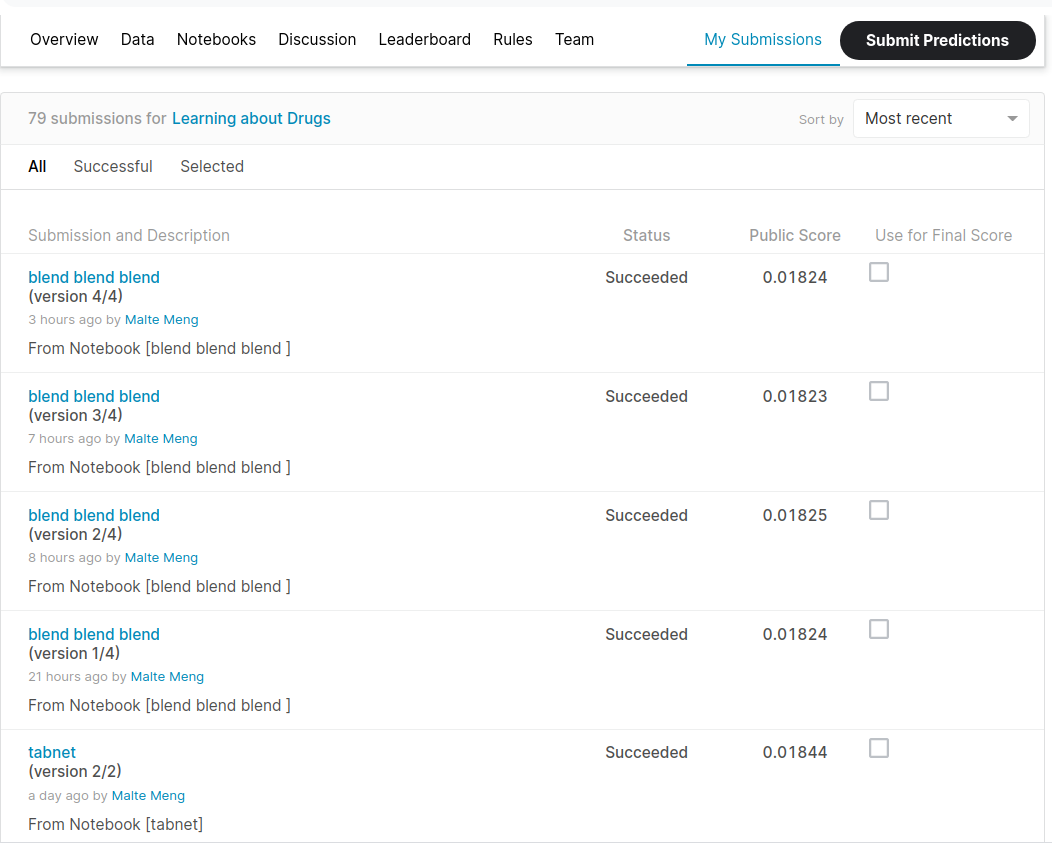
\includegraphics[width=1\textwidth]{pics/submissions.png}
    \caption{Results of submissions so far}
\label{fig:submissions}
\end{center}
\end{figure}

Evidence of leaderboard position on public dataset as of 21 Nov is shown in Figure \ref{fig:lb22nov}.
\begin{figure}[H]
\begin{center}
	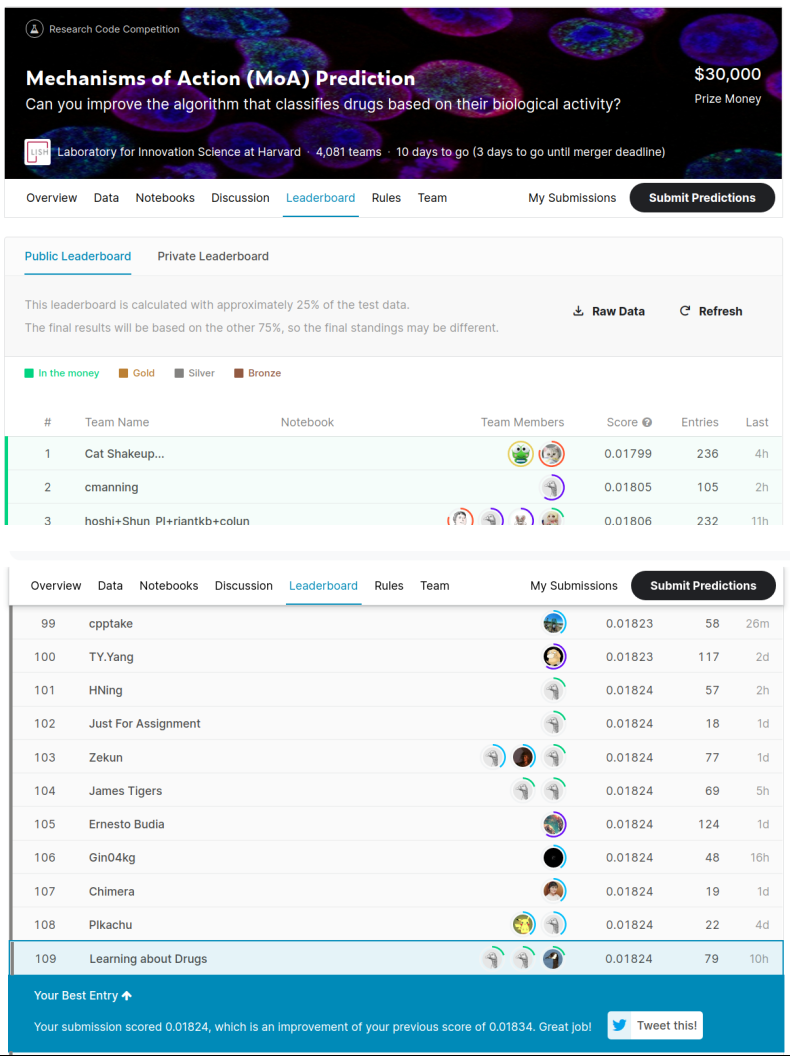
\includegraphics[width=1\textwidth]{pics/lb22nov.png}
    \caption{Leaderboard position as of 22 Nov}
\label{fig:lb22nov}
\end{center}
\end{figure}

\section{Ideas to try in next ten days}
\subsection{Model architectures}
\begin{enumerate}
    \item CNN-based architecture
    \item K-NN
    \item Autoencoder 
\end{enumerate}

\subsection{Pseudo-labelling}
Once we have a confident model prediction score for the public test dataset, we can include the public test data into our training set with the confidently predicted labels as the pseudo-ground truth, hopefully further boosting our scores.

\subsection{Model blending}
We could try more sophisticated methods of model blending, such as weighted averages and using optimisation to find the optimum weights and perhaps using a neural network with the predictions of several models as input and learning the best way to weight the different model predictions.

\bibliographystyle{IEEEtran} % We choose the "plain" reference style
\bibliography{ref} % Entries are in the "refs.bib" file

\end{document}